\chapter{Annex}
\setlength{\parskip}{2.5ex plus .4ex minus .4ex}
\section{Jobs}
\definecolor{cyan}{rgb}{0.7,0.7,1}
\noindent\begin{minipage}{\linewidth}% to keep image and caption on one page
\begin{center}
\begin{tabular}{| l | m{8cm} | c | c |}
\hline
	N & Title & Start & End\\\hline
	\rowcolor{cyan} L1 & Management & & \\
	T1	& Planning & S1 & S4\\
	T2	& Project monitoring & S5 & S24\\
	\rowcolor{cyan}L2 & SIGServer and agents integration & &\\
	T1	& Run SIGServer from ROS & S5 & S5\\
	T2	& Generation of one controller associated to one agent & S6 & S7\\
	T3	& Generation of controller for each agents & S8 & S8 \\
	\rowcolor{cyan}L3 & Make agents act & &\\
	T1	& Though Publish/Subscribe & S10 & S12\\
	T2	& Though ROS Services & S13 & S15\\
	\rowcolor{cyan}L4 & Services interface & &\\
	T1	& Design & S16 & S17\\
	T2	& Kinect & S18 & S20\\
	\rowcolor{cyan}L5 & Documentation & &\\
	T1	& Technical documentation & S5 & S18\\
	T2	& User documentation & S19& S23\\
	\rowcolor{cyan}L6 & Report & &\\
	T1	& Mid-term report & S8 & S9\\
	T2	& Final report & S22 & S24\\\hline
\end{tabular}
\end{center}
\captionof{table}{Jobs}\label{tab:lots}%      only if needed  
\end{minipage}

\begin{landscape}
\section{Schedule}\label{sec:schedule}
%\thispagestyle{empty}
%\thispagestyle{plain}
\setlength{\topmargin}{25pt}
\titlespacing{\subsection}{0cm}{0cm}{0cm}


\noindent\begin{ganttchart}[
hgrid,
vgrid,% = {*6{white}, *1{black}},% *{10}{blue, dashed}},
x unit=0.3cm,
%title/.style={fill=teal, draw=none},
%title label font=
%\color
%{white}
%\bfseries,
inline,
time slot format=isodate,
]{2015-03-16}{2015-06-07}
\gantttitlecalendar{year, month=name, week}{4} \\
\ganttbar{Planification}{2015-03-16}{2015-04-12}
\ganttbar{Project monitoring}{2015-04-13}{2015-06-07}\\

\ganttbar{DoW Report}{2015-04-03}{2015-04-12}
\ganttbar{Environment installation}{2015-03-16}{2015-03-28}
\ganttbar{Tutorials}{2015-03-29}{2015-04-02}
\ganttbar{L2:T1}{2015-04-13}{2015-04-19}
\ganttmilestone{DoW}{2015-04-12}
\ganttbar{L2:T2}{2015-04-20}{2015-05-03}
\ganttbar{L2:T3}{2015-05-04}{2015-05-10}
\ganttbar{L3:T1}{2015-05-18}{2015-06-07}\\

\ganttbar{Technical documentation}{2015-04-13}{2015-05-10}
\ganttbar{Technical documentation}{2015-05-18}{2015-06-07}\\

\ganttbar{Mid-term Report}{2015-05-04}{2015-05-17}
\ganttmilestone{Mid-term report}{2015-05-17}

\end{ganttchart}

\noindent\begin{ganttchart}[
hgrid,
vgrid,
x unit=0.3cm,
inline,
time slot format=isodate,
]{2015-06-08}{2015-08-30}
\gantttitlecalendar{month=name, week = 13} \\
\ganttbar{Project monitoring}{2015-06-08}{2015-08-30}\\
\ganttbar{L3:T2}{2015-06-08}{2015-06-28}
\ganttbar{L4:T1}{2015-06-29}{2015-07-12}
\ganttbar{L4:T2}{2015-07-13}{2015-08-02}
\ganttbar{Final Report}{2015-08-10}{2015-08-30}\ganttmilestone{Final Report}{2015-08-30}\\
\ganttbar{Technical documentation}{2015-06-08}{2015-08-02}
\ganttbar{User documentation}{2015-08-03}{2015-08-16}
\end{ganttchart}
\label{GanttChart}
\end{landscape}


\section{Topics}\label{annex:topics}
\begin{supertabular}{|p{2.9cm}|p{4.5cm}|p{7cm}|}
	\hline
    Topic name & Message & Description \\
  	\hline
  	\_onRecvMsg &
  		\textbf{sender} : string\newline 
  		\textbf{content} : string
  		\medskip & The ``Controller'' send the message received by the SIGViewer.\\
  	\hline
  	\medskip
  	\_onCollisionMsg &
  		\medskip
  		\textbf{name} : string \newline
  		\textbf{part} : string & The name of the agent which one is in collision with are sent to this topic. If there is severals collision at the same time, severals messages are sent.\\
  	\hline
  	\_setWheel & 
  		\textbf{wheelRadius} : double \newline
  		\textbf{wheelDistance} : double & Publish the radius and the distance in a message and they will be applied to the robot.\\
  	\hline
  	\_setWheelVelocity & 
  		\textbf{leftWheel} : double \newline
  		\textbf{rightWheel} : double
  		& Publish the velocity for the left and the right wheel and it will be applied.\\
  	\hline
  	\_setJointVelocity & 
  		\textbf{jointName} : string\newline
  		\textbf{angularVelocity} : double \newline
  		\textbf{max} : double
  		& jointName, angular velocity, max ???\\
  	\hline
  	\_releaseObj & \textbf{arm} : string & Publish the part which you want to release an object and it will be done.\\
  	\hline
  	\_setAxisAndAngle & 
  		\textbf{name} : string \newline
  		\textbf{axisX} : double \newline
  		\textbf{axisY} : double \newline
  		\textbf{axisZ} : double \newline
  		\textbf{angle} : double
  		& Set the axis defined by ``axisX'', ``axisY'' and ``axisZ'' and set the angle ``angle'' to the entity called ``name'', if no name is provided, the main entity of the topic will be set.\\
  	\hline
  	\_setPosition & 
  		\textbf{name} : string \newline
  		\textbf{posX} : double \newline
  		\textbf{posY} : double \newline
  		\textbf{posZ} : double
  		& Set the position ``posX'', ``posY'' and ``posZ'' to the entity called ``name'', if no name is provided, the main entity of the topic will be set.\\
  	\hline
\end{supertabular}

\section{Services}\label{annex:services}
\begin{supertabular}{|p{2.9cm}|p{2.5cm}|p{3cm}|p{5.5cm}|}
	\hline
    Service name & Request & Response & Description \\
  	\hline
  	\_get\_time &  & \textbf{time} : double & Get the simulation time.\\
  	\hline
  	\medskip
  	\_get\_obj\_position & \medskip \textbf{name} : string & 
  		\textbf{posX} : double \newline
  		\textbf{posY} : double \newline
  		\textbf{posZ} : double
  		 & Get the position of the object named name, if name is empty, return the position of the agent which the service's name start with.\\
  	\hline
  	\_get\_parts\_position & \textbf{part} : string & 
  		\begin{minipage}{3cm}
  			\medskip
  			\begin{description} 
  				\item[posX] : double 
  				\item[posY] : double 
  				\item[posZ] : double
  			\end{description}
  			\medskip
  		\end{minipage} & Get the position of the part in parameter.\\
  	\hline
  	\_get\_rotation & \textbf{axis} : string & 
  		\begin{minipage}{3cm}
  			\medskip
  			\begin{description} 
  				\item[qW] : double 
  				\item[qX] : double 
  				\item[qY] : double
  				\item[qZ] : double
  			\end{description}
  			\medskip
  		\end{minipage} & Get the rotation of ...\\
  	\hline
  	\_get\_angle\_rotation & 
  		\begin{minipage}{3cm}
  			\medskip
  			\begin{description} 
  				\item[axis] : string
  				\item[x] : double 
  				\item[y] : double 
  				\item[z] : double
  			\end{description}
  			\medskip
  		\end{minipage} & \textbf{angle} : double & Get the angle of ...\\
  	\hline
  	\_get\_joint\_angle & \textbf{nameArm} : string & \textbf{angle} : double & Get the angle between the joint.\\
  	\hline
  	\_grasp\_obj & 
  		\begin{minipage}{3cm}
  			\medskip
  			\begin{description} 
  				\item[part] : string
  				\item[obj] : string
  			\end{description}
  			\medskip
  		\end{minipage} & \textbf{ok} : bool & Grasp the object ``obj'' with the part ``part''\\
  	\hline
  	\_get\_entities & \textbf{axis} : string & 
  		\begin{minipage}{3cm}
  			\medskip
  			\begin{description} 
  				\item[entitiesNames] : string[] 
  				\item[length] : int
  			\end{description}
  			\medskip
  		\end{minipage} & Get the names of the entities in the simulator.\\
  	\hline
  	\_check\_service & \textbf{serviceName} : string & \textbf{connected} : bool & Check if the service ``serviceName'' is connected.\\
  	\hline
  	\_connect\_to\_service & \textbf{serviceName} : string & \textbf{connected} : bool & Connect the ``serviceName'', true if it is connected, false otherwise.\\
  	\hline
  	\_get\_collision\_state \_of\_main\_part & & \textbf{collisionState} : bool & Get the collision state of the main part.\\
  	\hline
  	\_is\_grasped & \textbf{entityName} : string & \textbf{answer} : bool & True if ``entityName'' is grasped, false otherwise. If no entity name is provided, it will return the answer for the agent which is asked\\
  	\hline
\end{supertabular}

%\section{pr2 tree}\label{annex:pr2Tree}
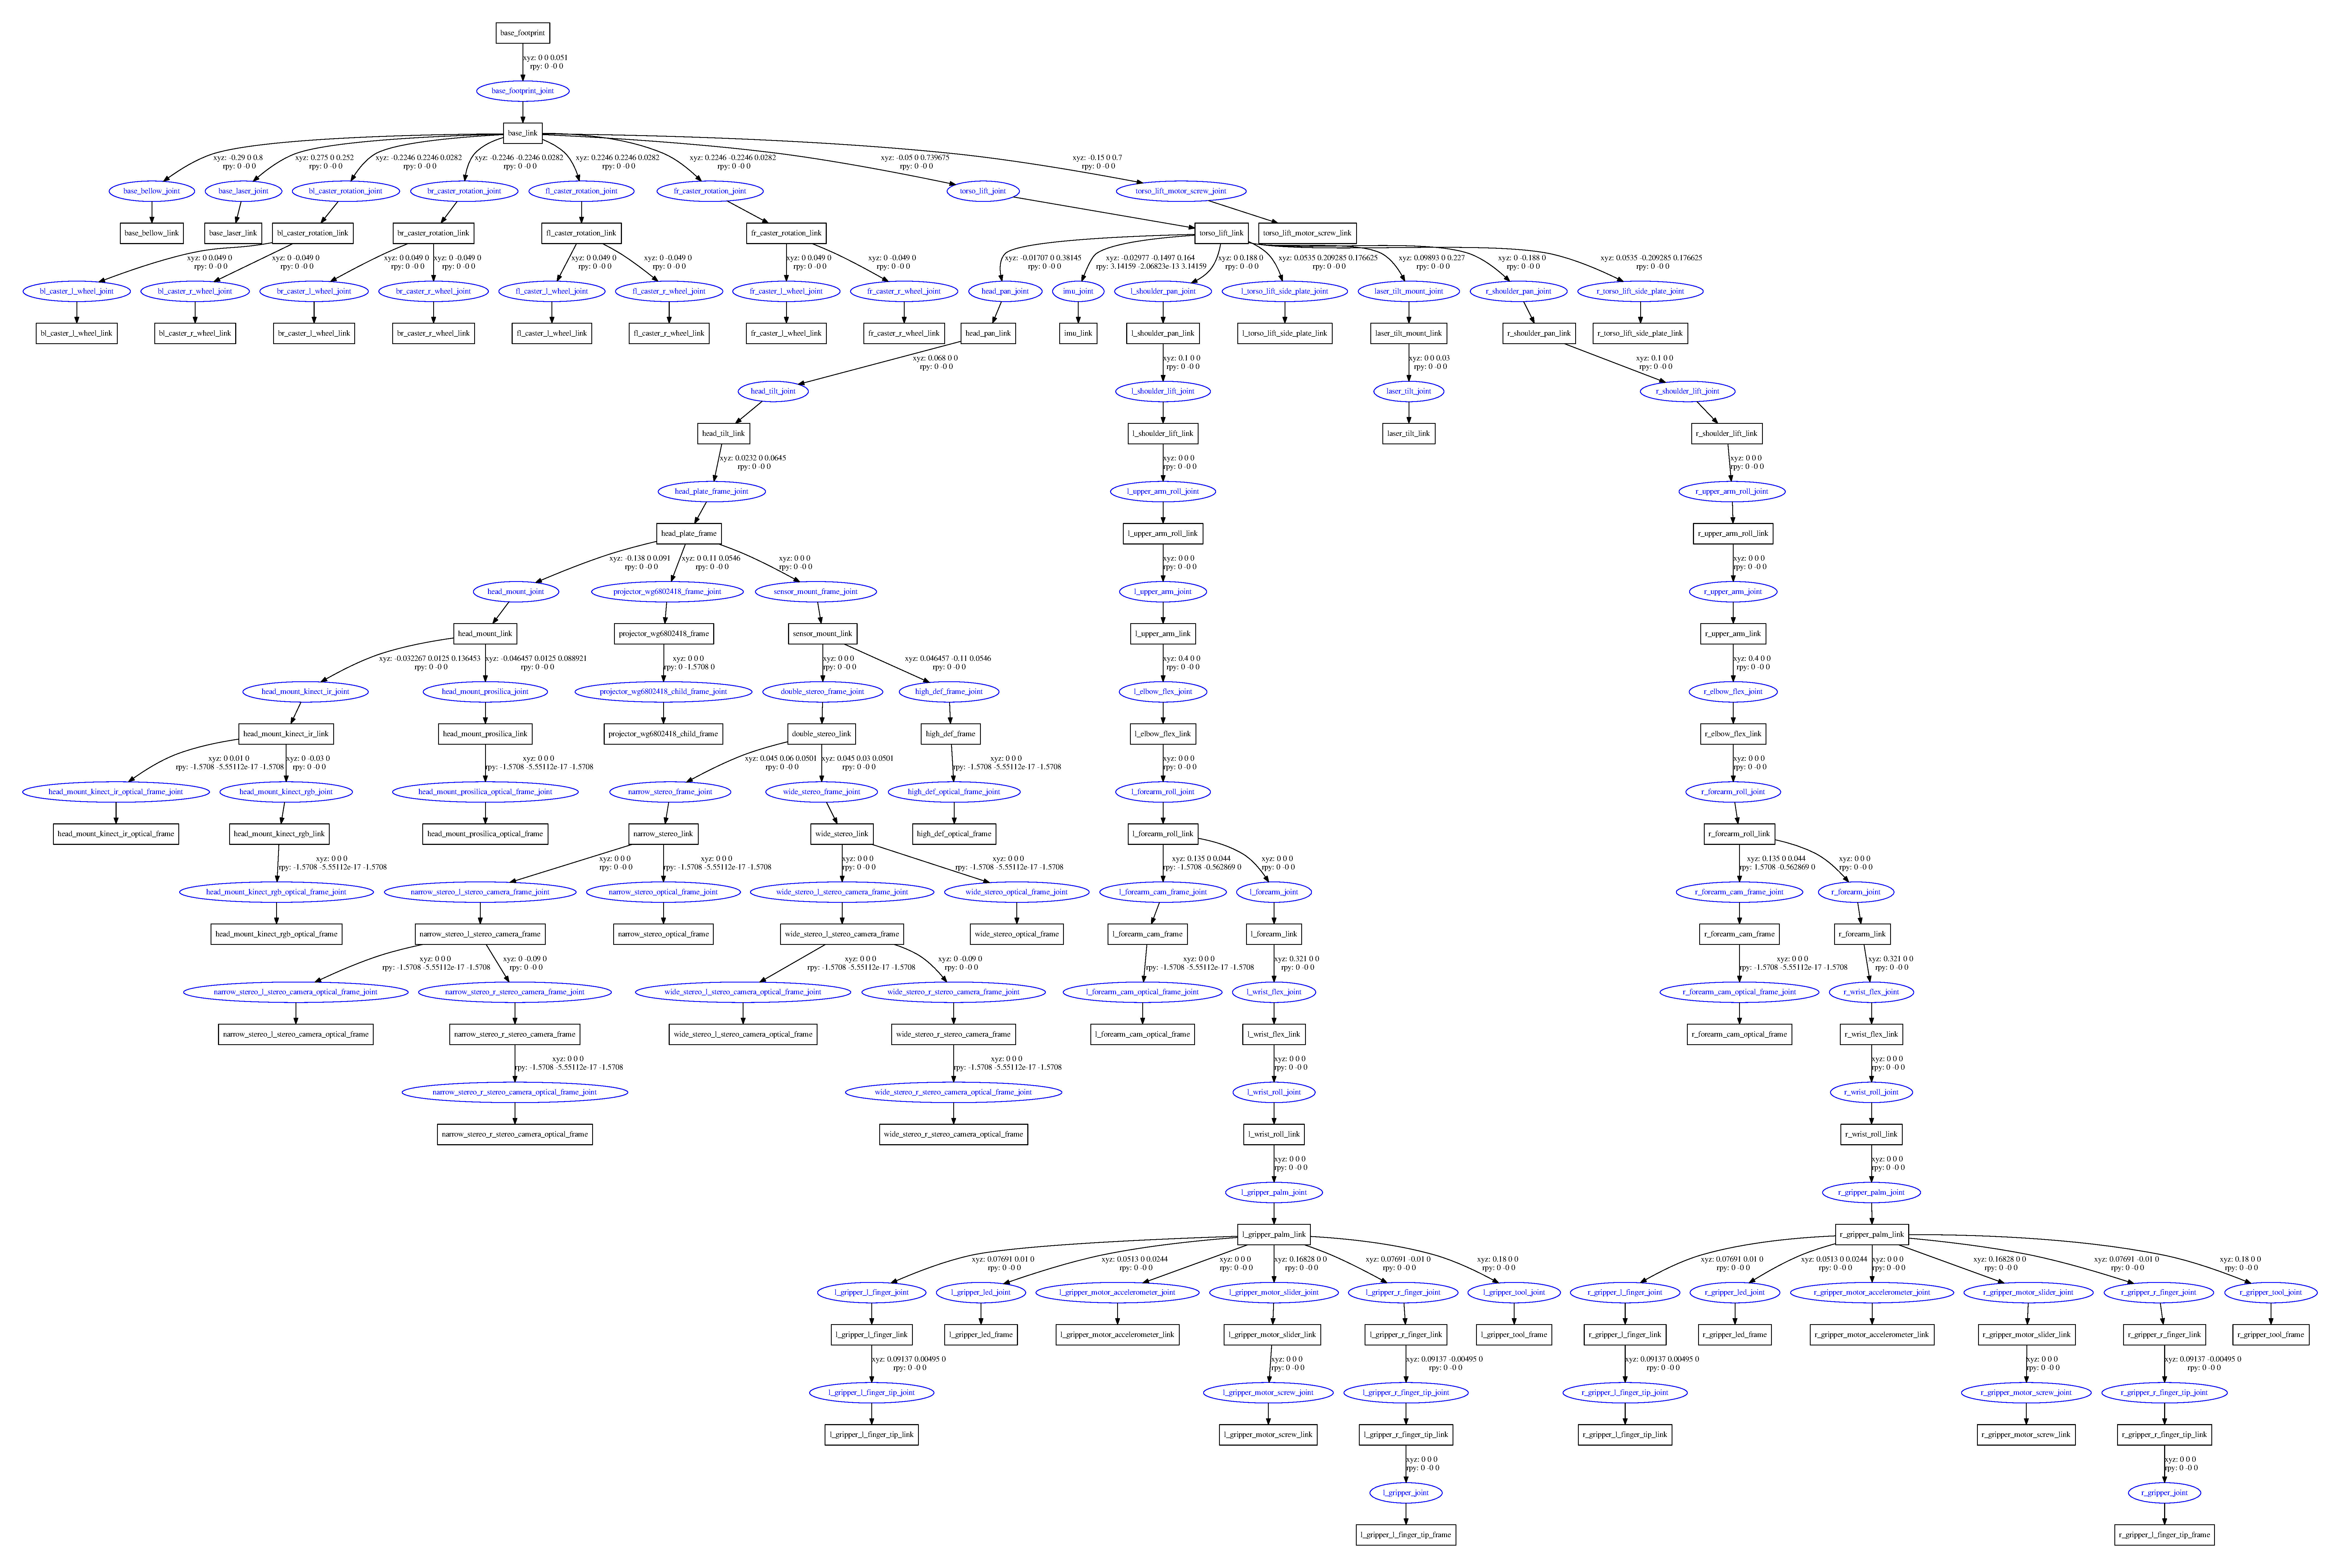
\includepdf[scale=0.95,pages=1,pagecommand=\section{Pr2 tree}\label{annex:pr2Tree}]{images/pr2Tree.pdf}
%\section{Minimal structure tree}\label{annex:minStruct}
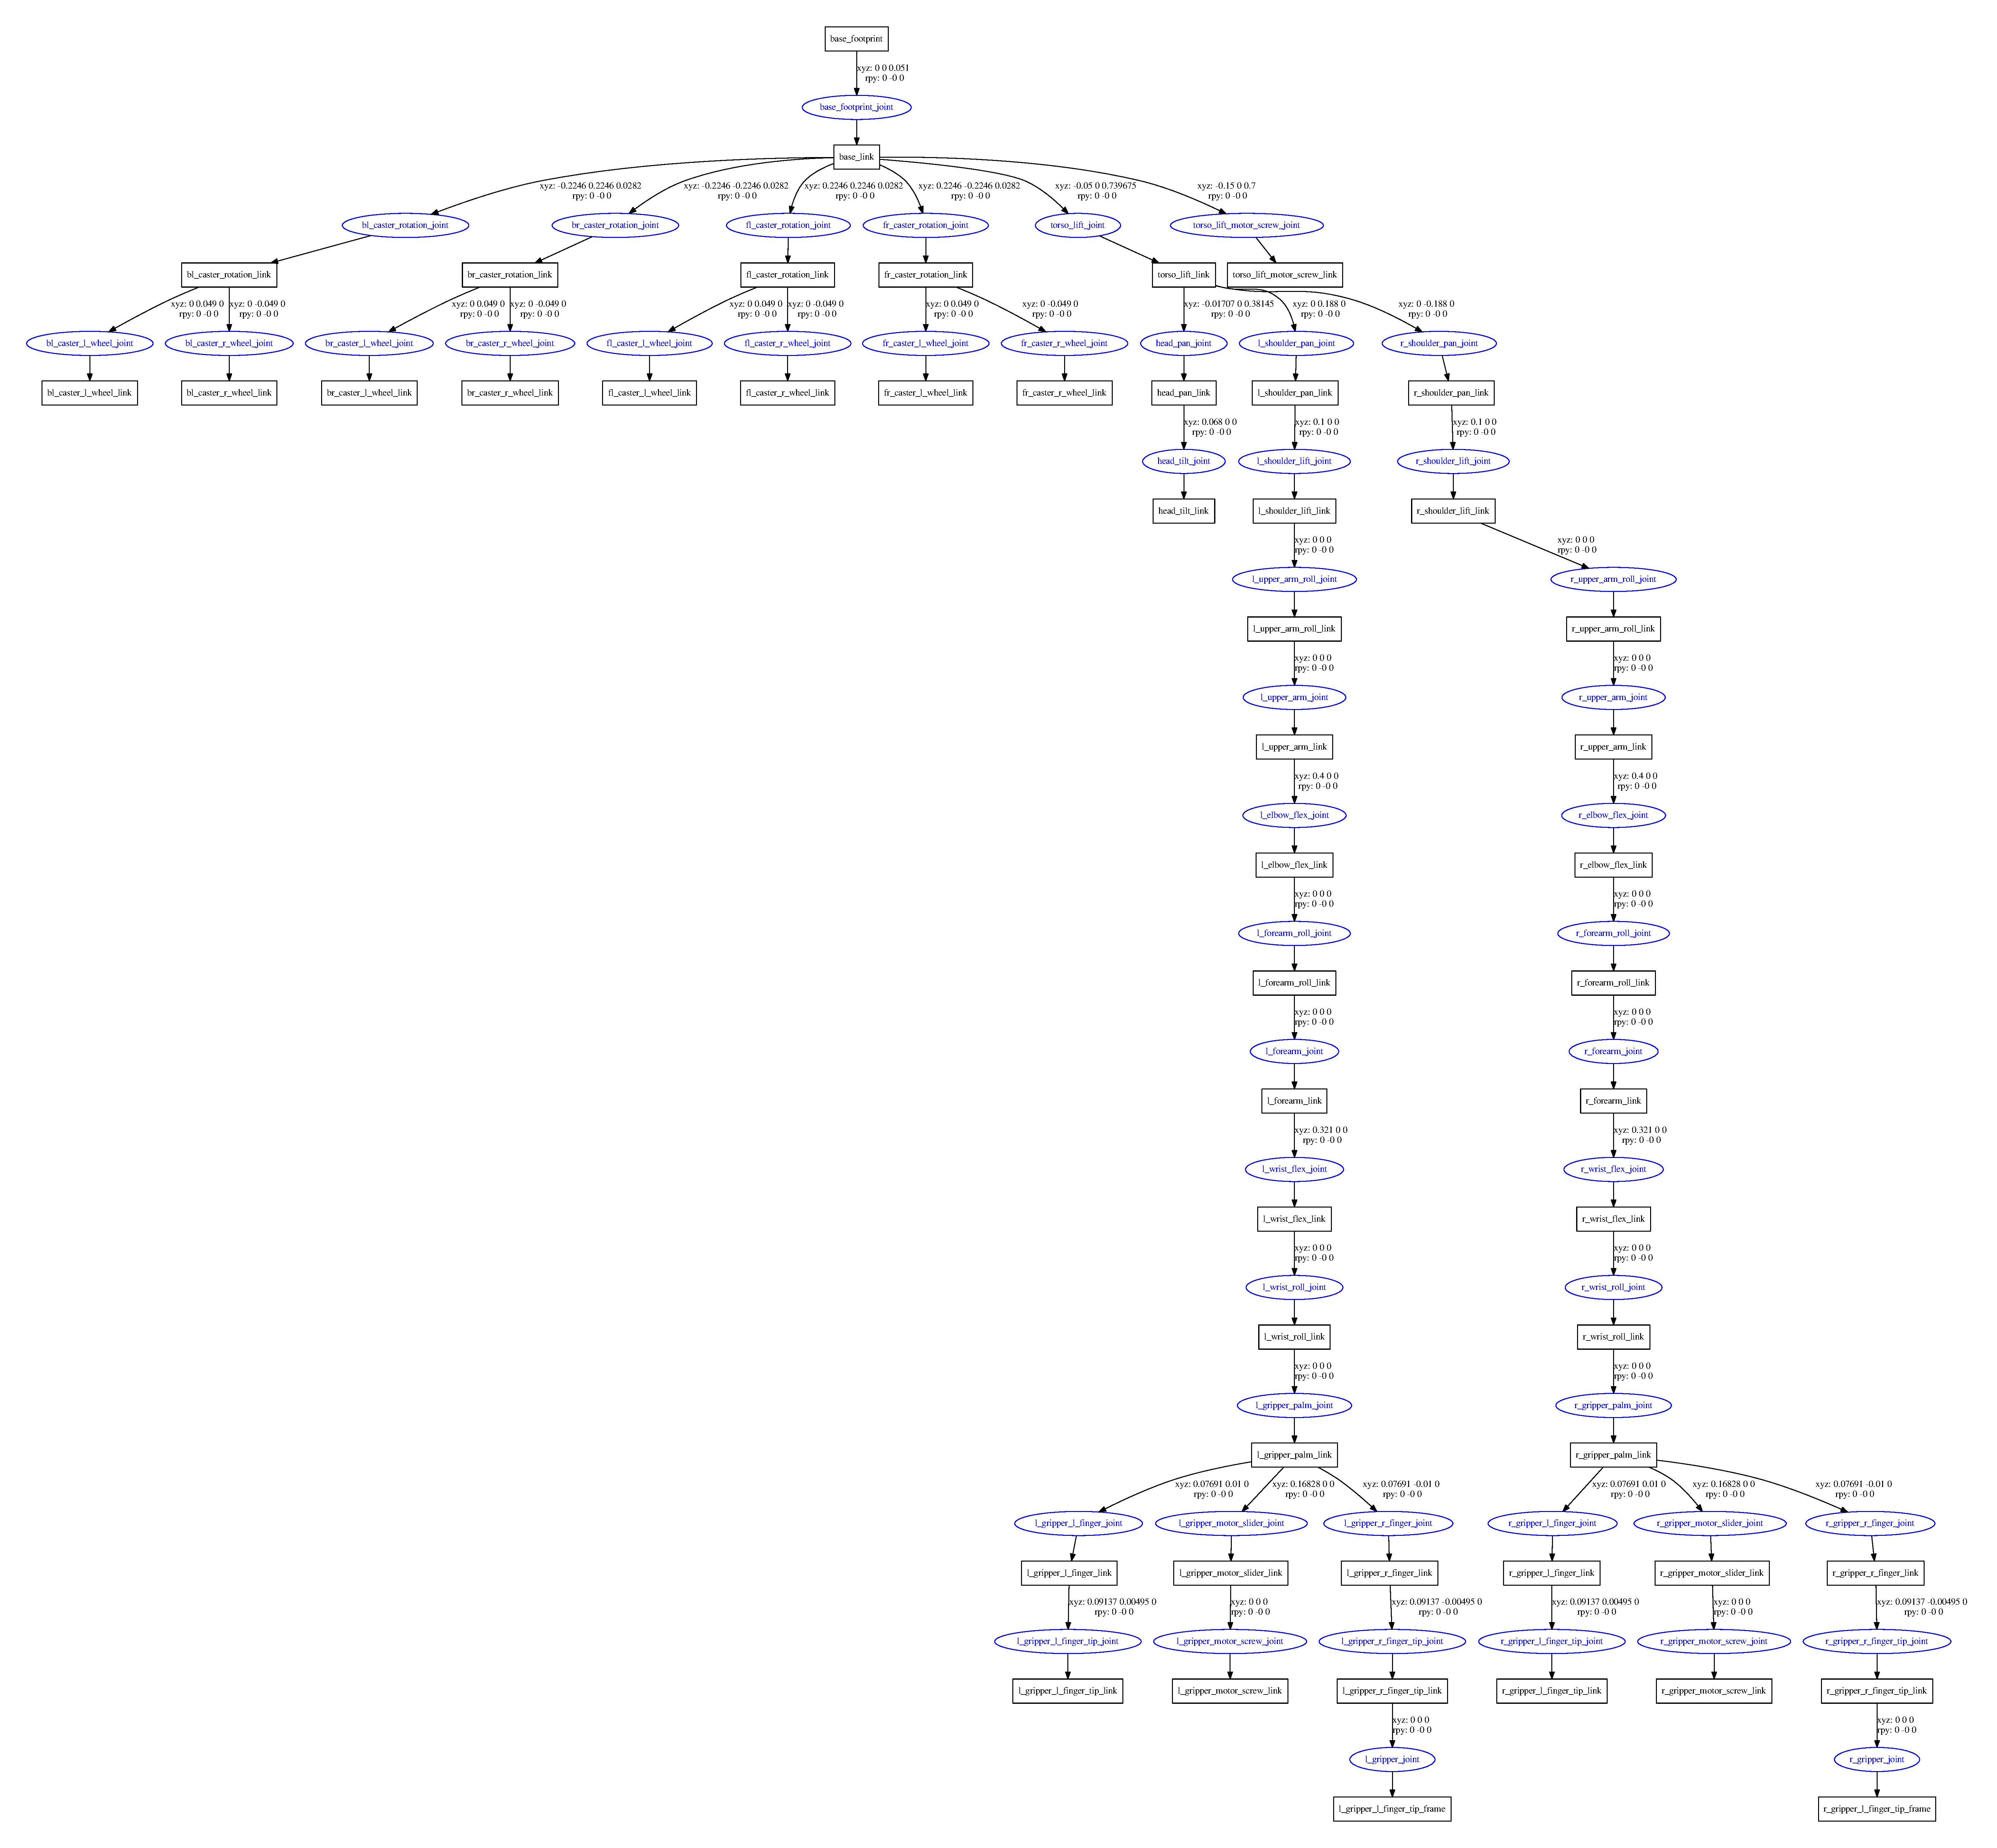
\includepdf[scale=0.95,pages=1,pagecommand=\section{Minimal structure tree}\label{annex:minStruct}]{images/bobbyTree.pdf}


\section{Position data of SIGVerse for an ik movement}\label{annex:dataPos}
\noindent\begin{minipage}{\linewidth}% to keep image and caption on one page
\begin{center}
\begin{tabular}{| l | m{8cm} | c | c |}
\hline
	Position asked & Result SIGVerse & Point name\\\hline
	0 0 -0.1 & 116.64 82.82 41.99 & B \\
	0 -0.1 0 & 116.64 93.83 43.51 & C\\
	0 0 0.05 & 116.64 99.20 41.39 & A\\
	0 0.15 0 & 116.64 93.98 44.83 & D\\
	0 -0.1 -0.1 & 116.64 82.93 43.59 & E\\
	0 -0.1 -0.15 & 116.64 77.59 43.16 & F\\
	0 -0.15 -0.1 & 116.64 83.18 45.33 & G\\
	0 0.1 0.03	& 116.64 97.05 43.05 & H\\
	0 0.16 0 & 116.64 94.24 44.91 & J\\
	0 -0.17 -0.1 & 116.64 83.56 46.09 & K\\
	0 0 -0.08 & 116.64 85.05 42.13 & L\\
	0 0 -0.05 & 116.64 88.38 42.22 & M\\\hline
\end{tabular}
\end{center}
\captionof{table}{Jobs}\label{tab:lots}%      only if needed  
\end{minipage}